\section{A multi-mission site pack}
\label{sec:data}

\begin{figure*}[t]
  \centering
  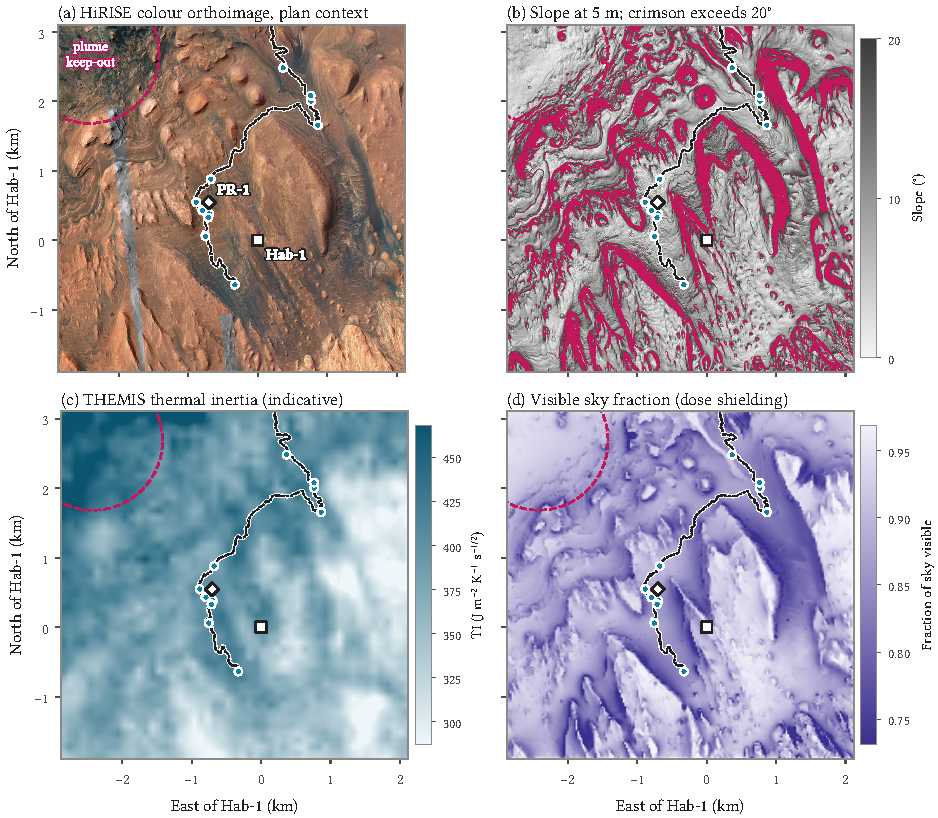
\includegraphics[width=0.6\textwidth]{site.pdf}
  \caption{The Gale study area (5\,km\,$\times$\,5\,km) in the \code{gale-v1} site pack, in kilometres relative to the scenario habitat. Dotted line: Curiosity's traverse; cyan dots: the twelve candidate stations; square: Hab-1; diamond: PR-1; dashed circle: 1\,km landing-plume keep-out. (a) HiRISE colour orthoimage. (b) Slope at 5\,m from the USGS merged DEM; 22.5\% of cells exceed $20^\circ$ (crimson). (c) THEMIS thermal inertia, an indicative terrain factor. (d) Fraction of sky visible from 1\,m above the ground, used for terrain shielding of the dose.}
  \label{fig:site}
\end{figure*}

Our site is a 5\,km\,$\times$\,5\,km area on the lower slopes of Aeolis Mons in Gale crater, centred at \ang{137.388}\,E, \ang{4.805}\,S. It covers Curiosity's 2023--26 traverse, including the ``boxwork'' ridges studied in 2025--26 \citep{thompson2025boxwork,siebach2025boxwork} (\cref{fig:site}). The site is the challenge's own example. Curiosity's waypoints give surveyed positions for checking the terrain model, and RAD measurements of terrain shielding there let us test our dose model \citep{guo2026}. The twelve candidate stations are real Curiosity targets, each positioned from the rover's waypoint on the sol it was studied (\cref{app:stations}, \cref{tab:stations}). The habitat, rover and landing-zone positions are scenario assumptions placed by a documented siting heuristic, not NASA selections. The scenario is sol 412 of a notional crewed mission, at 09:40 local true solar time (LTST).

The terrain is the USGS merged Gale digital elevation model (DEM), which combines HiRISE stereo models with CTX, HRSC and MOLA elevations at 1\,m posting \citep{parker2016galedem,mcewen2007,malin2007,jaumann2007,smith2001}. It drives which cells are walkable, step grade and length, walking energy, radio line of sight, sun relief and the pressure used for dose. THEMIS thermal inertia \citep{christensen2004,fergason2006} sets an indicative terrain factor in the walking cost. CRISM summary parameters \citep{murchie2007,viviano2014} give sulfate and hydration signals at each stop. Curiosity's traverse, Mastcam and Navcam images \citep{grotzinger2012,malin2017,maki2012}, REMS weather \citep{gomezelvira2012} and RAD dose data \citep{hassler2012} supply ground truth, point-of-view images and conditions. WSA--ENLIL coronal-mass-ejection forecasts come from NASA's DONKI service \citep{odstrcil2003,arge2000,donki}, and sun geometry from Mars24 \citep{allison2000}. \Cref{tab:layers} in \cref{app:tables} lists every layer, its product and its role.

All layers share one 1,000\,$\times$\,1,000 grid in a local equidistant cylindrical projection on the IAU Mars sphere of radius 3,396,190\,m \citep{archinal2018}. The sources are equirectangular on the same sphere, so reprojection is an exact affine operation. Slope uses Horn's method \citep{horn1981hill}. A popular web-map library computes ground distance on an Earth-sized sphere by default, which would draw every Mars scale bar 1.88 times too long; \Marswalk overrides this and pins the fix with a unit test. Against Curiosity's localized elevations at 372 waypoints, the DEM differs by a median of $-0.001$\,m with a standard deviation of 0.19\,m. Both products are tied to HiRISE, so this measures consistency rather than independent accuracy. The CRISM product sat about 270\,m from the same features in HiRISE, and after a rigid correction the residuals are 10--30\,m. Every pack is checked against its schema and SHA-256 digests.

The pipeline is site-agnostic. A second pack covers the western delta front of Jezero crater, built from the USGS Mars 2020 terrain-relative-navigation DTM and orthomosaic \citep{fergason2020trn} and Perseverance data \citep{farley2020}. Its DEM differs from 220 Perseverance waypoints with a standard deviation of 0.07\,m. The engine, console and navigator run on it unchanged.
